%%%%%%%%%%%%%%%%%%%%%%%%%%%%%%%%%%%%%%%%%
% University/School Laboratory Report
% LaTeX Template
% Version 3.1 (25/3/14)
%
% This template has been downloaded from:
% http://www.LaTeXTemplates.com
%
% Original author:
% Linux and Unix Users Group at Virginia Tech Wiki 
% (https://vtluug.org/wiki/Example_LaTeX_chem_lab_report)
%
% License:
% CC BY-NC-SA 3.0 (http://creativecommons.org/licenses/by-nc-sa/3.0/)
%
%%%%%%%%%%%%%%%%%%%%%%%%%%%%%%%%%%%%%%%%%

%----------------------------------------------------------------------------------------
%	PACKAGES AND DOCUMENT CONFIGURATIONS
%----------------------------------------------------------------------------------------

\documentclass[12pt]{article}

%\usepackage[version=3]{mhchem} % Package for chemical equation typesetting
%\usepackage{siunitx} % Provides the \SI{}{} and \si{} command for typesetting SI units
\usepackage[left=1in,top=1in,right=1in,bottom=1in]{geometry} % Document margins
\usepackage{graphicx} % Required for the inclusion of images
\usepackage{pdfpages}
\usepackage{natbib} % Required to change bibliography style to APA
\usepackage{amsmath} % Required for some math elements 

\setlength\parindent{0pt} % Removes all indentation from paragraphs

\renewcommand{\labelenumi}{\alph{enumi}.} % Make numbering in the enumerate environment by letter rather than number (e.g. section 6)

%\usepackage{times} % Uncomment to use the Times New Roman font

%----------------------------------------------------------------------------------------
%	DOCUMENT INFORMATION
%----------------------------------------------------------------------------------------

\title{\textbf{Find A Room} \\ Design Document \\ CS 307} % Title

\author{Team \textsc{13}(Snoxy)} % Author name

\date{\today} % Date for the report

\begin{document}

\maketitle % Insert the title, author and date

\begin{center}
\begin{tabular}{l r}
Members: & Nathan Chang \\ % Partner names
& Xiaojing Ji \\
& Zilun Mai(Owen) \\
& \textbf{Saranyu Phusit(Team Leader)} \\
& Yao Xiao \\
\\
\bigskip
Instructor: & Professor Buster Dunsmore \\% Instructor/supervisor 
Project Coordinator: & Miguel Villarreal-Vasquez % Instructor/supervisor

\end{tabular}
\end{center}

\newpage
\tableofcontents

% If you wish to include an abstract, uncomment the lines below
% \begin{abstract}
% Abstract text
% \end{abstract}

%----------------------------------------------------------------------------------------
%	SECTION 1
%----------------------------------------------------------------------------------------


\newpage
\section{Purpose}

A mobile application that will give directions indoors by scanning QR codes put on walls throughout a building. The app will direct them towards their destination from where they are.


\section{Design Outline}

\subsection{Requirements}
The design should meet the following requirements.

\begin{itemize}
\item Having a visual guide with photos for navigating me to destination.
\item Navigating to the closest restrooms and water fountains and other destinations.
\item Getting the current location.
\item Automation adding my building map into an app and specify important destinations at ease. 
\item Response Time: The response time after user starts walking should not be more than 1 second

\end{itemize}

\subsection{General Priority}
The decisions that we make in this document are based on the priorities that we have set for the
project. These are (in order of importance):
\begin{itemize}
\item \textbf{Reliability:} The app should lead the user to the destination as quickly and precisely as possible. We take it seriously since that's the most important part of our project.
\item \textbf{Scalability:} The app should work with any building with basic structure.
\item \textbf{Size:} The size of the app should be small, the user should download it quickly.
\item \textbf{Supportability:} The app should work without having the developers add the map and checkpoints manually. We may add it if time allows.
\end{itemize}

\subsection{Outline Figures}

Lorem ipsum dolor sit amet, consectetuer adipiscing elit. Aenean commodo ligula eget dolor. Aenean massa. Cum sociis natoque penatibus et magnis dis parturient montes, nascetur ridiculus mus. Donec quam felis, ultricies nec, pellentesque eu, pretium quis, sem. Nulla consequat massa quis enim. Donec pede justo, fringilla vel, aliquet nec, vulputate eget, arcu. In enim justo, rhoncus ut, imperdiet a, venenatis vitae, justo. Nullam dictum felis eu pede mollis pretium. Integer tincidunt. Cras dapibus. Vivamus elementum semper nisi. Aenean vulputate eleifend tellus. Aenean leo ligula, porttitor eu, consequat vitae, eleifend ac, enim. Aliquam lorem ante, dapibus in, viverra quis, feugiat a, tellus. Phasellus viverra nulla ut metus varius laoreet. Quisque rutrum. Aenean imperdiet. Etiam ultricies nisi vel augue. Curabitur ullamcorper ultricies nisi. Nam eget dui. Etiam rhoncus. Maecenas tempus, tellus eget condimentum rhoncus, sem quam semper libero, sit amet adipiscing sem neque sed ipsum. Nam quam nunc, blandit vel, luctus pulvinar, hendrerit id, lorem. Maecenas nec odio et ante tincidunt tempus. Donec vitae sapien ut libero venenatis faucibus. Nullam quis ante. Etiam sit amet orci eget eros faucibus tincidunt. Duis leo. Sed fringilla mauris sit amet nibh. Donec sodales sagittis magna. Sed consequat, leo eget bibendum sodales, augue velit cursus nunc,

\begin{center}
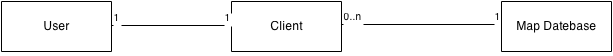
\includegraphics[scale=0.8]{image/user_outline.png}
\end{center}



\section{Design Issue}

We run into several issues.

\subsection{Functional Issue}
\subsubsection{Issue 1}

Where to put QR Code. \\ \\

Option 1: On every destination \\
Option 2: On the corner of the building \\

Although Option 1 will make the path-finding easier, we still decide to use option 2 since the user won’t go through the wrong way when on an edge, and it is a waste of time to put all the QR code on the wall.

\subsubsection{Issue 2}
How should user get the map database? \\ \\

Option 1: Download it with the app. \\
Option 2: Download when user want it. \\

We choose Option 1 since when user needs to use it, he or she must be in hurry of finding a classroom or bathroom so he or she may not have time to download it. 



\subsection{Non-functional Issue}
Mobile app or Website app? \\ \\
Option 1: Mobile \\
Option 2: Webapp \\ \\

We choose option 2 since we can use XXX to transfer to a mobile program and it doesn't need native support for iOS/Andriod.

\subsubsection{Issue X}
Lorem ipsum dolor sit amet, consectetuer adipiscing elit. Aenean commodo ligula eget dolor. Aenean massa. Cum sociis natoque penatibus et magnis dis parturient montes, nascetur ridiculus mus. Donec quam felis, ultricies nec, pellentesque eu, pretium quis, sem. Nulla consequat massa quis enim. Donec pede justo, fringilla vel, aliquet nec, vulputate eget, arcu. In enim justo, rhoncus ut, imperdiet a, venenatis vitae, justo. Nullam dictum felis eu pede mollis pretium. Integer tincidunt. Cras dapibus. Vivamus elementum semper nisi. Aenean vulputate eleifend tellus. Aenean leo ligula, porttitor eu, consequat vitae, eleifend ac, enim. Aliquam lorem ante, dapibus in, viverra quis, feugiat a, tellus. Phasellus viverra nulla ut metus varius laoreet. Quisque rutrum. Aenean imperdiet. Etiam ultricies nisi vel augue. Curabitur ullamcorper ultricies nisi. Nam eget dui. Etiam rhoncus. Maecenas tempus, tellus eget condimentum rhoncus, sem quam semper libero, sit amet adipiscing sem neque sed ipsum. Nam quam nunc, blandit vel, luctus pulvinar, hendrerit id, lorem. Maecenas nec odio et ante tincidunt tempus. Donec vitae sapien ut libero venenatis faucibus. Nullam quis ante. Etiam sit amet orci eget eros faucibus tincidunt. Duis leo. Sed fringilla mauris sit amet nibh. Donec sodales sagittis magna. Sed consequat, leo eget bibendum sodales, augue velit cursus nunc,



\section{Design Details}
In order to achieve successful indoor navigation, the designing of this project will consider the database storing locations of lecture rooms, rest rooms and water fountain, as well as the way of locating users and navigating them to destinations inside the building.  
We decide to apply QR code and link each QR code to a specific location of maps. Maps has a real map images and a list of nodes and edges which represents the map abstractly.  To generate graph of the map, every single node indicates a room, andi every edge(with direction) means the length between two nodes. The graph is a connection of nodes and edges.  The first image of following class diagram provides more details of it.
	
\subsection{Components}
\textbf{QRcode:}
	Each QR code stores its own ID. It will use QR code ID to find the corresponding map, so that users can locate themselves and obtain the floor map by simply scanning and sending the QR code to our app
\\ \\
\textbf{Map: }
	Each map can be identified by its own ID named MapID. Since the real map is translated to graph, rooms and water fountains are represented by nodes, the paths between two neighborhoods are represented by edges. NodeList stores every node displayed on the map, as well as EdgeList stores every edge with direction.  MapImg holds the real life map for better user visualization.  The MapImg will be pumped out on the screen once the app successfully identify user’s location and load the corresponding map.
\\ \\ For ComputeMap(), once the system gets user’s location and destination on the map, this method helps calculate the total distance by summing up the edges(path in real life) among nodes(rooms and public facilities in real) that user will pass. The summation can be done by method addNode() and addEdge(). Thus, each single map contains multiple nodes and edges, but it can only generate one optimized path formed by those nodes and edges.
\\ \\
\textbf{Path:}
	Since every time user can only pick up one destination, eventually the system will provide only one path from current location to destination, this class keeps edges formed that path in a list.
\\ \\

\textbf{Node:}
Each node can be distinguished by its own NodeID, IsRoom is a boolean variable to recognize whether the node is a lecture room or public facilities. PosX and PosY record the location of that node, in order to help locate each node on the map to find the optimized path.  
\\ 

\textbf{Edge:}
Edges all have their own ID called EdgeID, and their starting and ending nodes. This object helps ComputePath() to find the path.
\\ \\
\textbf{Destination:}
Destination is parsed from user’s selection on the lecture rooms list, or public facilities. Each of them can be identified by it DestinationID. 
\begin{center}
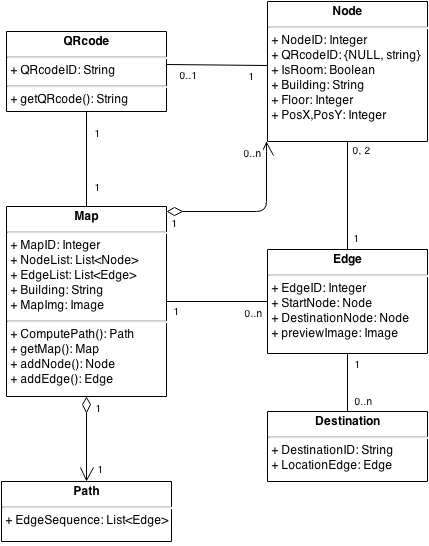
\includegraphics[scale=0.6]{image/image01.png}
\\
\textit{Figure 1. The Class diagram}
\end{center}
\subsection{Process}
We have two main process for this project. The user should scan the QR code and get the location of the current position, as well as providing the destination. The client should provide directions and showing the map of the current area.

\begin{center}
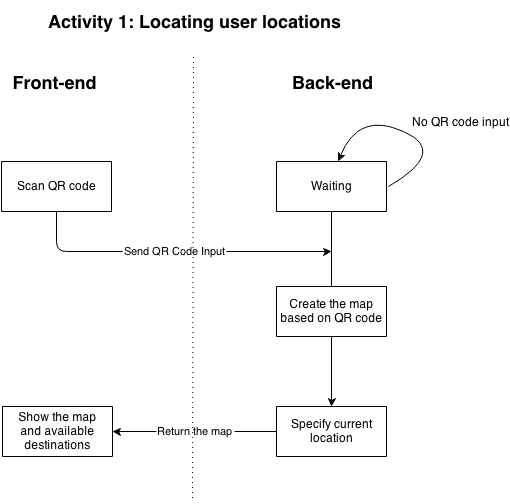
\includegraphics[scale=0.6]{image/image00.png}
\end{center}

\begin{center}
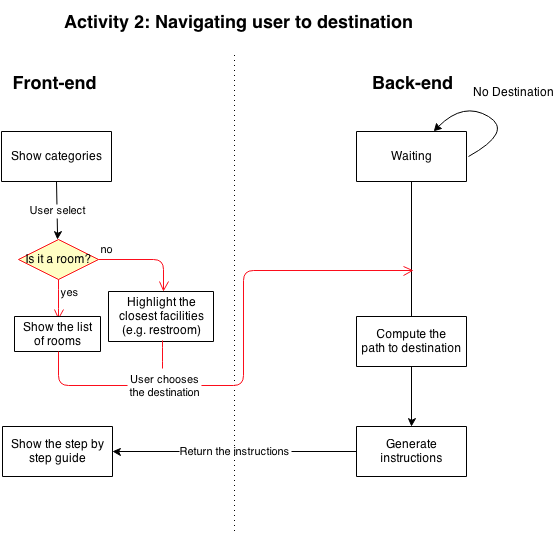
\includegraphics[scale=0.6]{image/image02.png}
\end{center}




\subsection{UI mockup}
Lorem ipsum dolor sit amet, consectetuer adipiscing elit. Aenean commodo ligula eget dolor. Aenean massa. Cum sociis natoque penatibus et magnis dis parturient montes, nascetur ridiculus mus. Donec quam felis, ultricies nec, pellentesque eu, pretium quis, sem. Nulla consequat massa quis enim. Donec pede justo, fringilla vel, aliquet nec, vulputate eget, arcu. In enim justo, rhoncus ut, imperdiet a, venenatis vitae, justo. Nullam dictum felis eu pede mollis pretium. Integer tincidunt. Cras dapibus. Vivamus elementum semper nisi. Aenean vulputate eleifend tellus. Aenean leo ligula, porttitor eu, consequat vitae, eleifend ac, enim. Aliquam lorem ante, dapibus in, viverra quis, feugiat a, tellus. Phasellus viverra nulla ut metus varius laoreet. Quisque rutrum. Aenean imperdiet. Etiam ultricies nisi vel augue. Curabitur ullamcorper ultricies nisi. Nam eget dui. Etiam rhoncus. Maecenas tempus, tellus eget condimentum rhoncus, sem quam semper libero, sit amet adipiscing sem neque sed ipsum. Nam quam nunc, blandit vel, luctus pulvinar, hendrerit id, lorem. Maecenas nec odio et ante tincidunt tempus. Donec vitae sapien ut libero venenatis faucibus. Nullam quis ante. Etiam sit amet orci eget eros faucibus tincidunt. Duis leo. Sed fringilla mauris sit amet nibh. Donec sodales sagittis magna. Sed consequat, leo eget bibendum sodales, augue velit cursus nunc,


Lorem ipsum dolor sit amet, consectetuer adipiscing elit. Aenean commodo ligula eget dolor. Aenean massa. Cum sociis natoque penatibus et magnis dis parturient montes, nascetur ridiculus mus. Donec quam felis, ultricies nec, pellentesque eu, pretium quis, sem. Nulla consequat massa quis enim. Donec pede justo, fringilla vel, aliquet nec, vulputate eget, arcu. In enim justo, rhoncus ut, imperdiet a, venenatis vitae, justo. Nullam dictum felis eu pede mollis pretium. Integer tincidunt. Cras dapibus. Vivamus elementum semper nisi. Aenean vulputate eleifend tellus. Aenean leo ligula, porttitor eu, consequat vitae, eleifend ac, enim. Aliquam lorem ante, dapibus in, viverra quis, feugiat a, tellus. Phasellus viverra nulla ut metus varius laoreet. Quisque rutrum. Aenean imperdiet. Etiam ultricies nisi vel augue. Curabitur ullamcorper ultricies nisi. Nam eget dui. Etiam rhoncus. Maecenas tempus, tellus eget condimentum rhoncus, sem quam semper libero, sit amet adipiscing sem neque sed ipsum. Nam quam nunc, blandit vel, luctus pulvinar, hendrerit id, lorem. Maecenas nec odio et ante tincidunt tempus. Donec vitae sapien ut libero venenatis faucibus. Nullam quis ante. Etiam sit amet orci eget eros faucibus tincidunt. Duis leo. Sed fringilla mauris sit amet nibh. Donec sodales sagittis magna. Sed consequat, leo eget bibendum sodales, augue velit cursus nunc,


\end{document}